\documentclass[aspectratio=169]{beamer}
\usetheme{simple}

\RequirePackage[l2tabu, orthodox]{nag}


% \usepackage[left=1.in, right=1.in, top=1.25in, bottom=1.25in]{geometry}

% FONTS
%\usepackage[T1]{fontenc}

% Replace default Latin Modern typewriter with its proportional counterpart
% http://www.tug.dk/FontCatalogue/lmoderntypewriterprop/
%\renewcommand*\ttdefault{lmvtt}


%%% OPTION 1 - Fourier Math + New Century Schoolbook + ParaType Sans

% % Import Fourier Math (this imposes its own New Century Schoolbook type)
% % http://www.ctan.org/tex-archive/fonts/fouriernc/
%\usepackage{fouriernc}
%\usepackage{amsmath}
% % Replace with TeX Gyre Schola version of New Century Schoolbook (must scale!)
% % http://www.tug.dk/FontCatalogue/tgschola/
%\usepackage[scale=0.92]{tgschola}
%\usepackage[scaled=0.88]{PTSans}

%% OPTION 2 - MathDesign Math + Bitstream Charter + ParaType Sans

% Import MathDesign (this brings along Bitstream Charter)
% http://www.ctan.org/tex-archive/fonts/mathdesign/
\usepackage[bitstream-charter]{mathdesign}
\usepackage{amsmath}
\usepackage[scaled=0.92]{PTSans}


% %%% OPTION 3 - MTPRO 2 Math + Termes Times + ParaType Sans

% \usepackage{tgtermes}
% \usepackage{amsmath}
% \usepackage[subscriptcorrection,
%             amssymbols,
%             mtpbb,
%             mtpcal,
%             nofontinfo  % suppresses all warnings
%            ]{mtpro2}
% \usepackage{scalefnt,letltxmacro}
% \LetLtxMacro{\oldtextsc}{\textsc}
% \renewcommand{\textsc}[1]{\oldtextsc{\scalefont{1.10}#1}}
% \usepackage[scaled=0.92]{PTSans}

% Use default fonts here
\usepackage{amsmath}
\usepackage{amssymb}

% \usepackage{titling}

% % COLOR
% \usepackage[table,usenames,dvipsnames]{xcolor}
\definecolor{shadecolor}{gray}{0.9}

% SPACING and TEXT
\usepackage[final,expansion=alltext]{microtype}
\usepackage[english]{babel}
\usepackage[parfill]{parskip}
\usepackage{afterpage}
\usepackage{framed}
\usepackage{verbatim}
\usepackage{setspace}

\newenvironment{exercise}[1]
{
    \itshape
    \paragraph{Exercise: \textit{#1}}
}
{ 
}


% \usepackage[bottom]{footmisc}
\usepackage[symbol]{footmisc}
\renewcommand{\thefootnote}{\arabic{footnote}}


% FIGURES
\usepackage{graphicx}
\usepackage[labelfont={it, small}, 
            textfont={small,singlespacing},
            % justification={justified,RaggedRight},
            singlelinecheck=false,
            margin=0pt]{caption}
\usepackage[format=hang]{subcaption}
% \usepackage{ccaption}

% % APPENDIX FIGURES
% \usepackage{chngcntr}

% % TABLES
% \usepackage{booktabs}
% \usepackage{longtable}
% \usepackage{hhline}

% ALGORITHMS
\usepackage[algoruled]{algorithm2e}
\usepackage{listings}
\usepackage{fancyvrb}
\fvset{fontsize=\normalsize}

% % THEOREMS
\usepackage{amsthm}
\newtheorem{proposition}{Proposition}
% \newtheorem{lemma}{Lemma}

% % BIBLIOGRAPHY
\usepackage{natbib}

% HYPERREF
% \usepackage[colorlinks,linktoc=all]{hyperref}
% \usepackage[all]{hypcap}
% \hypersetup{citecolor=MidnightBlue}
% \hypersetup{linkcolor=black}
% \hypersetup{urlcolor=MidnightBlue}

% % CLEVEREF must come after HYPERREF
% \usepackage[nameinlink]{cleveref}

% % ACRONYMS
% \usepackage[acronym,smallcaps,nowarn]{glossaries}
% % \makeglossaries

% % COLOR DEFINITIONS
\newcommand{\red}[1]{\textcolor{BrickRed}{#1}}
\newcommand{\orange}[1]{\textcolor{BurntOrange}{#1}}
\newcommand{\green}[1]{\textcolor{OliveGreen}{#1}}
\newcommand{\blue}[1]{\textcolor{MidnightBlue}{#1}}
\newcommand{\gray}[1]{\textcolor{black!60}{#1}}

% LISTINGS DEFINTIONS
\lstdefinestyle{mystyle}{
    commentstyle=\color{OliveGreen},
    keywordstyle=\color{BurntOrange},
    numberstyle=\tiny\color{black!60},
    stringstyle=\color{MidnightBlue},
    basicstyle=\ttfamily,
    breakatwhitespace=false,
    breaklines=true,
    captionpos=b,
    keepspaces=true,
    numbers=left,
    numbersep=5pt,
    showspaces=false,
    showstringspaces=false,
    showtabs=false,
    tabsize=2
}
\lstset{style=mystyle}

\usepackage[colorinlistoftodos,
            prependcaption,
            textsize=small,
            backgroundcolor=yellow,
            linecolor=lightgray,
            bordercolor=lightgray]{todonotes}

\usepackage{soul}

\usepackage{media9}
% !TEX root = template.tex

% \DeclareRobustCommand{\mb}[1]{\ensuremath{\boldsymbol{\mathbf{#1}}}}
\DeclareRobustCommand{\mb}[1]{\boldsymbol{#1}}

% \newcommand{\KL}[2]{\ensuremath{\textrm{KL}\PARENS{#1\;\|\;#2}}}
\DeclareRobustCommand{\KL}[2]{\ensuremath{\textrm{KL}\left(#1\;\|\;#2\right)}}

\DeclareMathOperator*{\argmax}{arg\,max}
\DeclareMathOperator*{\argmin}{arg\,min}

\renewcommand{\mid}{~\vert~}
\newcommand{\given}{\,|\,}
\newcommand{\iid}[1]{\stackrel{\text{iid}}{#1}}

\newcommand{\mba}{\mb{a}}
\newcommand{\mbb}{\mb{b}}
\newcommand{\mbc}{\mb{c}}
\newcommand{\mbd}{\mb{d}}
\newcommand{\mbe}{\mb{e}}
% \newcommand{\mbf}{\mb{f}}
\newcommand{\mbg}{\mb{g}}
\newcommand{\mbh}{\mb{h}}
\newcommand{\mbi}{\mb{i}}
\newcommand{\mbj}{\mb{j}}
\newcommand{\mbk}{\mb{k}}
\newcommand{\mbl}{\mb{l}}
\newcommand{\mbm}{\mb{m}}
\newcommand{\mbn}{\mb{n}}
\newcommand{\mbo}{\mb{o}}
\newcommand{\mbp}{\mb{p}}
\newcommand{\mbq}{\mb{q}}
\newcommand{\mbr}{\mb{r}}
\newcommand{\mbs}{\mb{s}}
\newcommand{\mbt}{\mb{t}}
\newcommand{\mbu}{\mb{u}}
\newcommand{\mbv}{\mb{v}}
\newcommand{\mbw}{\mb{w}}
\newcommand{\mbx}{\mb{x}}
\newcommand{\mby}{\mb{y}}
\newcommand{\mbz}{\mb{z}}

\newcommand{\mbA}{\mb{A}}
\newcommand{\mbB}{\mb{B}}
\newcommand{\mbC}{\mb{C}}
\newcommand{\mbD}{\mb{D}}
\newcommand{\mbE}{\mb{E}}
\newcommand{\mbF}{\mb{F}}
\newcommand{\mbG}{\mb{G}}
\newcommand{\mbH}{\mb{H}}
\newcommand{\mbI}{\mb{I}}
\newcommand{\mbJ}{\mb{J}}
\newcommand{\mbK}{\mb{K}}
\newcommand{\mbL}{\mb{L}}
\newcommand{\mbM}{\mb{M}}
\newcommand{\mbN}{\mb{N}}
\newcommand{\mbO}{\mb{O}}
\newcommand{\mbP}{\mb{P}}
\newcommand{\mbQ}{\mb{Q}}
\newcommand{\mbR}{\mb{R}}
\newcommand{\mbS}{\mb{S}}
\newcommand{\mbT}{\mb{T}}
\newcommand{\mbU}{\mb{U}}
\newcommand{\mbV}{\mb{V}}
\newcommand{\mbW}{\mb{W}}
\newcommand{\mbX}{\mb{X}}
\newcommand{\mbY}{\mb{Y}}
\newcommand{\mbZ}{\mb{Z}}

\newcommand{\mbalpha}{\mb{\alpha}}
\newcommand{\mbbeta}{\mb{\beta}}
\newcommand{\mbdelta}{\mb{\delta}}
\newcommand{\mbepsilon}{\mb{\epsilon}}
\newcommand{\mbchi}{\mb{\chi}}
\newcommand{\mbeta}{\mb{\eta}}
\newcommand{\mbgamma}{\mb{\gamma}}
\newcommand{\mbiota}{\mb{\iota}}
\newcommand{\mbkappa}{\mb{\kappa}}
\newcommand{\mblambda}{\mb{\lambda}}
\newcommand{\mbmu}{\mb{\mu}}
\newcommand{\mbnu}{\mb{\nu}}
\newcommand{\mbomega}{\mb{\omega}}
\newcommand{\mbphi}{\mb{\phi}}
\newcommand{\mbpi}{\mb{\pi}}
\newcommand{\mbpsi}{\mb{\psi}}
\newcommand{\mbrho}{\mb{\rho}}
\newcommand{\mbsigma}{\mb{\sigma}}
\newcommand{\mbtau}{\mb{\tau}}
\newcommand{\mbtheta}{\mb{\theta}}
\newcommand{\mbupsilon}{\mb{\upsilon}}
\newcommand{\mbvarepsilon}{\mb{\varepsilon}}
\newcommand{\mbvarphi}{\mb{\varphi}}
\newcommand{\mbvartheta}{\mb{\vartheta}}
\newcommand{\mbvarrho}{\mb{\varrho}}
\newcommand{\mbxi}{\mb{\xi}}
\newcommand{\mbzeta}{\mb{\zeta}}

\newcommand{\mbDelta}{\mb{\Delta}}
\newcommand{\mbGamma}{\mb{\Gamma}}
\newcommand{\mbLambda}{\mb{\Lambda}}
\newcommand{\mbOmega}{\mb{\Omega}}
\newcommand{\mbPhi}{\mb{\Phi}}
\newcommand{\mbPi}{\mb{\Pi}}
\newcommand{\mbPsi}{\mb{\Psi}}
\newcommand{\mbSigma}{\mb{\Sigma}}
\newcommand{\mbTheta}{\mb{\Theta}}
\newcommand{\mbUpsilon}{\mb{\Upsilon}}
\newcommand{\mbXi}{\mb{\Xi}}

\newcommand{\dif}{\mathop{}\!\mathrm{d}}
\newcommand{\diag}{\textrm{diag}}
\newcommand{\supp}{\textrm{supp}}
\newcommand{\Tr}{\textrm{Tr}}

\newcommand{\E}{\mathbb{E}}
\newcommand{\Var}{\mathbb{V}\textrm{ar}}
% \newcommand{\given}{\mid}

\newcommand{\bbA}{\mathbb{A}}
\newcommand{\bbB}{\mathbb{B}}
\newcommand{\bbC}{\mathbb{C}}
\newcommand{\bbD}{\mathbb{D}}
\newcommand{\bbE}{\mathbb{E}}
\newcommand{\bbF}{\mathbb{F}}
\newcommand{\bbG}{\mathbb{G}}
\newcommand{\bbH}{\mathbb{H}}
\newcommand{\bbI}{\mathbb{I}}
\newcommand{\bbJ}{\mathbb{J}}
\newcommand{\bbK}{\mathbb{K}}
\newcommand{\bbL}{\mathbb{L}}
\newcommand{\bbM}{\mathbb{M}}
\newcommand{\bbN}{\mathbb{N}}
\newcommand{\bbO}{\mathbb{O}}
\newcommand{\bbP}{\mathbb{P}}
\newcommand{\bbQ}{\mathbb{Q}}
\newcommand{\bbR}{\mathbb{R}}
\newcommand{\bbS}{\mathbb{S}}
\newcommand{\bbT}{\mathbb{T}}
\newcommand{\bbU}{\mathbb{U}}
\newcommand{\bbV}{\mathbb{V}}
\newcommand{\bbW}{\mathbb{W}}
\newcommand{\bbX}{\mathbb{X}}
\newcommand{\bbY}{\mathbb{Y}}
\newcommand{\bbZ}{\mathbb{Z}}

\newcommand{\cA}{\mathcal{A}}
\newcommand{\cB}{\mathcal{B}}
\newcommand{\cC}{\mathcal{C}}
\newcommand{\cD}{\mathcal{D}}
\newcommand{\cE}{\mathcal{E}}
\newcommand{\cF}{\mathcal{F}}
\newcommand{\cG}{\mathcal{G}}
\newcommand{\cH}{\mathcal{H}}
\newcommand{\cI}{\mathcal{I}}
\newcommand{\cJ}{\mathcal{J}}
\newcommand{\cK}{\mathcal{K}}
\newcommand{\cL}{\mathcal{L}}
\newcommand{\cM}{\mathcal{M}}
\newcommand{\cN}{\mathcal{N}}
\newcommand{\cO}{\mathcal{O}}
\newcommand{\cP}{\mathcal{P}}
\newcommand{\cQ}{\mathcal{Q}}
\newcommand{\cR}{\mathcal{R}}
\newcommand{\cS}{\mathcal{S}}
\newcommand{\cT}{\mathcal{T}}
\newcommand{\cU}{\mathcal{U}}
\newcommand{\cV}{\mathcal{V}}
\newcommand{\cW}{\mathcal{W}}
\newcommand{\cX}{\mathcal{X}}
\newcommand{\cY}{\mathcal{Y}}
\newcommand{\cZ}{\mathcal{Z}}

\newcommand{\trans}{\mathsf{T}}
\newcommand{\naturals}{\mathbb{N}}
\newcommand{\reals}{\mathbb{R}}
\newcommand{\const}{\mathrm{const}}

\newcommand{\distBernoulli}{\mathrm{Bern}}
\newcommand{\distBeta}{\mathrm{Beta}}
\newcommand{\distBinomial}{\mathrm{Bin}}
\newcommand{\distCategorical}{\mathrm{Cat}}
\newcommand{\distDirichlet}{\mathrm{Dir}}
\newcommand{\distExp}{\mathrm{Exp}}
\newcommand{\distGamma}{\mathrm{Gamma}}
\newcommand{\distMNIW}{\mathrm{MNIW}}
\newcommand{\distMultinomial}{\mathrm{Mult}}
\newcommand{\distNegBinomial}{\mathrm{NB}}
\newcommand{\distNormal}{\mathcal{N}}
\newcommand{\distPoisson}{\mathrm{Po}}
\newcommand{\distPoissonProcess}{\mathrm{PP}}
\newcommand{\distPolyaGamma}{\mathrm{PG}}
\newcommand{\distUniform}{\mathrm{Unif}}
\newcommand{\distInvChiSq}{\mathrm{Inv-}\chi^2}

\newcommand{\dtmax}{\Delta t_{\mathsf{max}}}

\newcommand{\mbzero}{\boldsymbol{0}}
% \newacronym{KL}{kl}{Kullback-Leibler}
\newacronym{ELBO}{elbo}{\emph{evidence lower bound}}
\newacronym{EM}{em}{\emph{expectation-maximization}}
\newacronym{PPCA}{ppca}{probabilistic principal components analysis}

\newacronym{SVI}{svi}{stochastic variational inference}
\newacronym{GMM}{gmm}{Gaussian mixture model}
\newacronym{HMM}{hmm}{hidden Markov model}
\newacronym{IO-HMM}{io-hmm}{input-output hidden Markov model}
\newacronym{LDS}{lds}{linear dynamical system}
\newacronym{SLDS}{slds}{switching linear dynamical system}
\newacronym{AR-HMM}{ar-hmm}{autoregressive hidden Markov model}


\title{STATS271/371: Applied Bayesian Statistics}
\subtitle{Mixed Membership Models, Topic Models, and Variational Inference}
\author{Scott Linderman}
\date{\today}


\begin{document}


\maketitle

\begin{frame}{Box's Loop}
\begin{center}
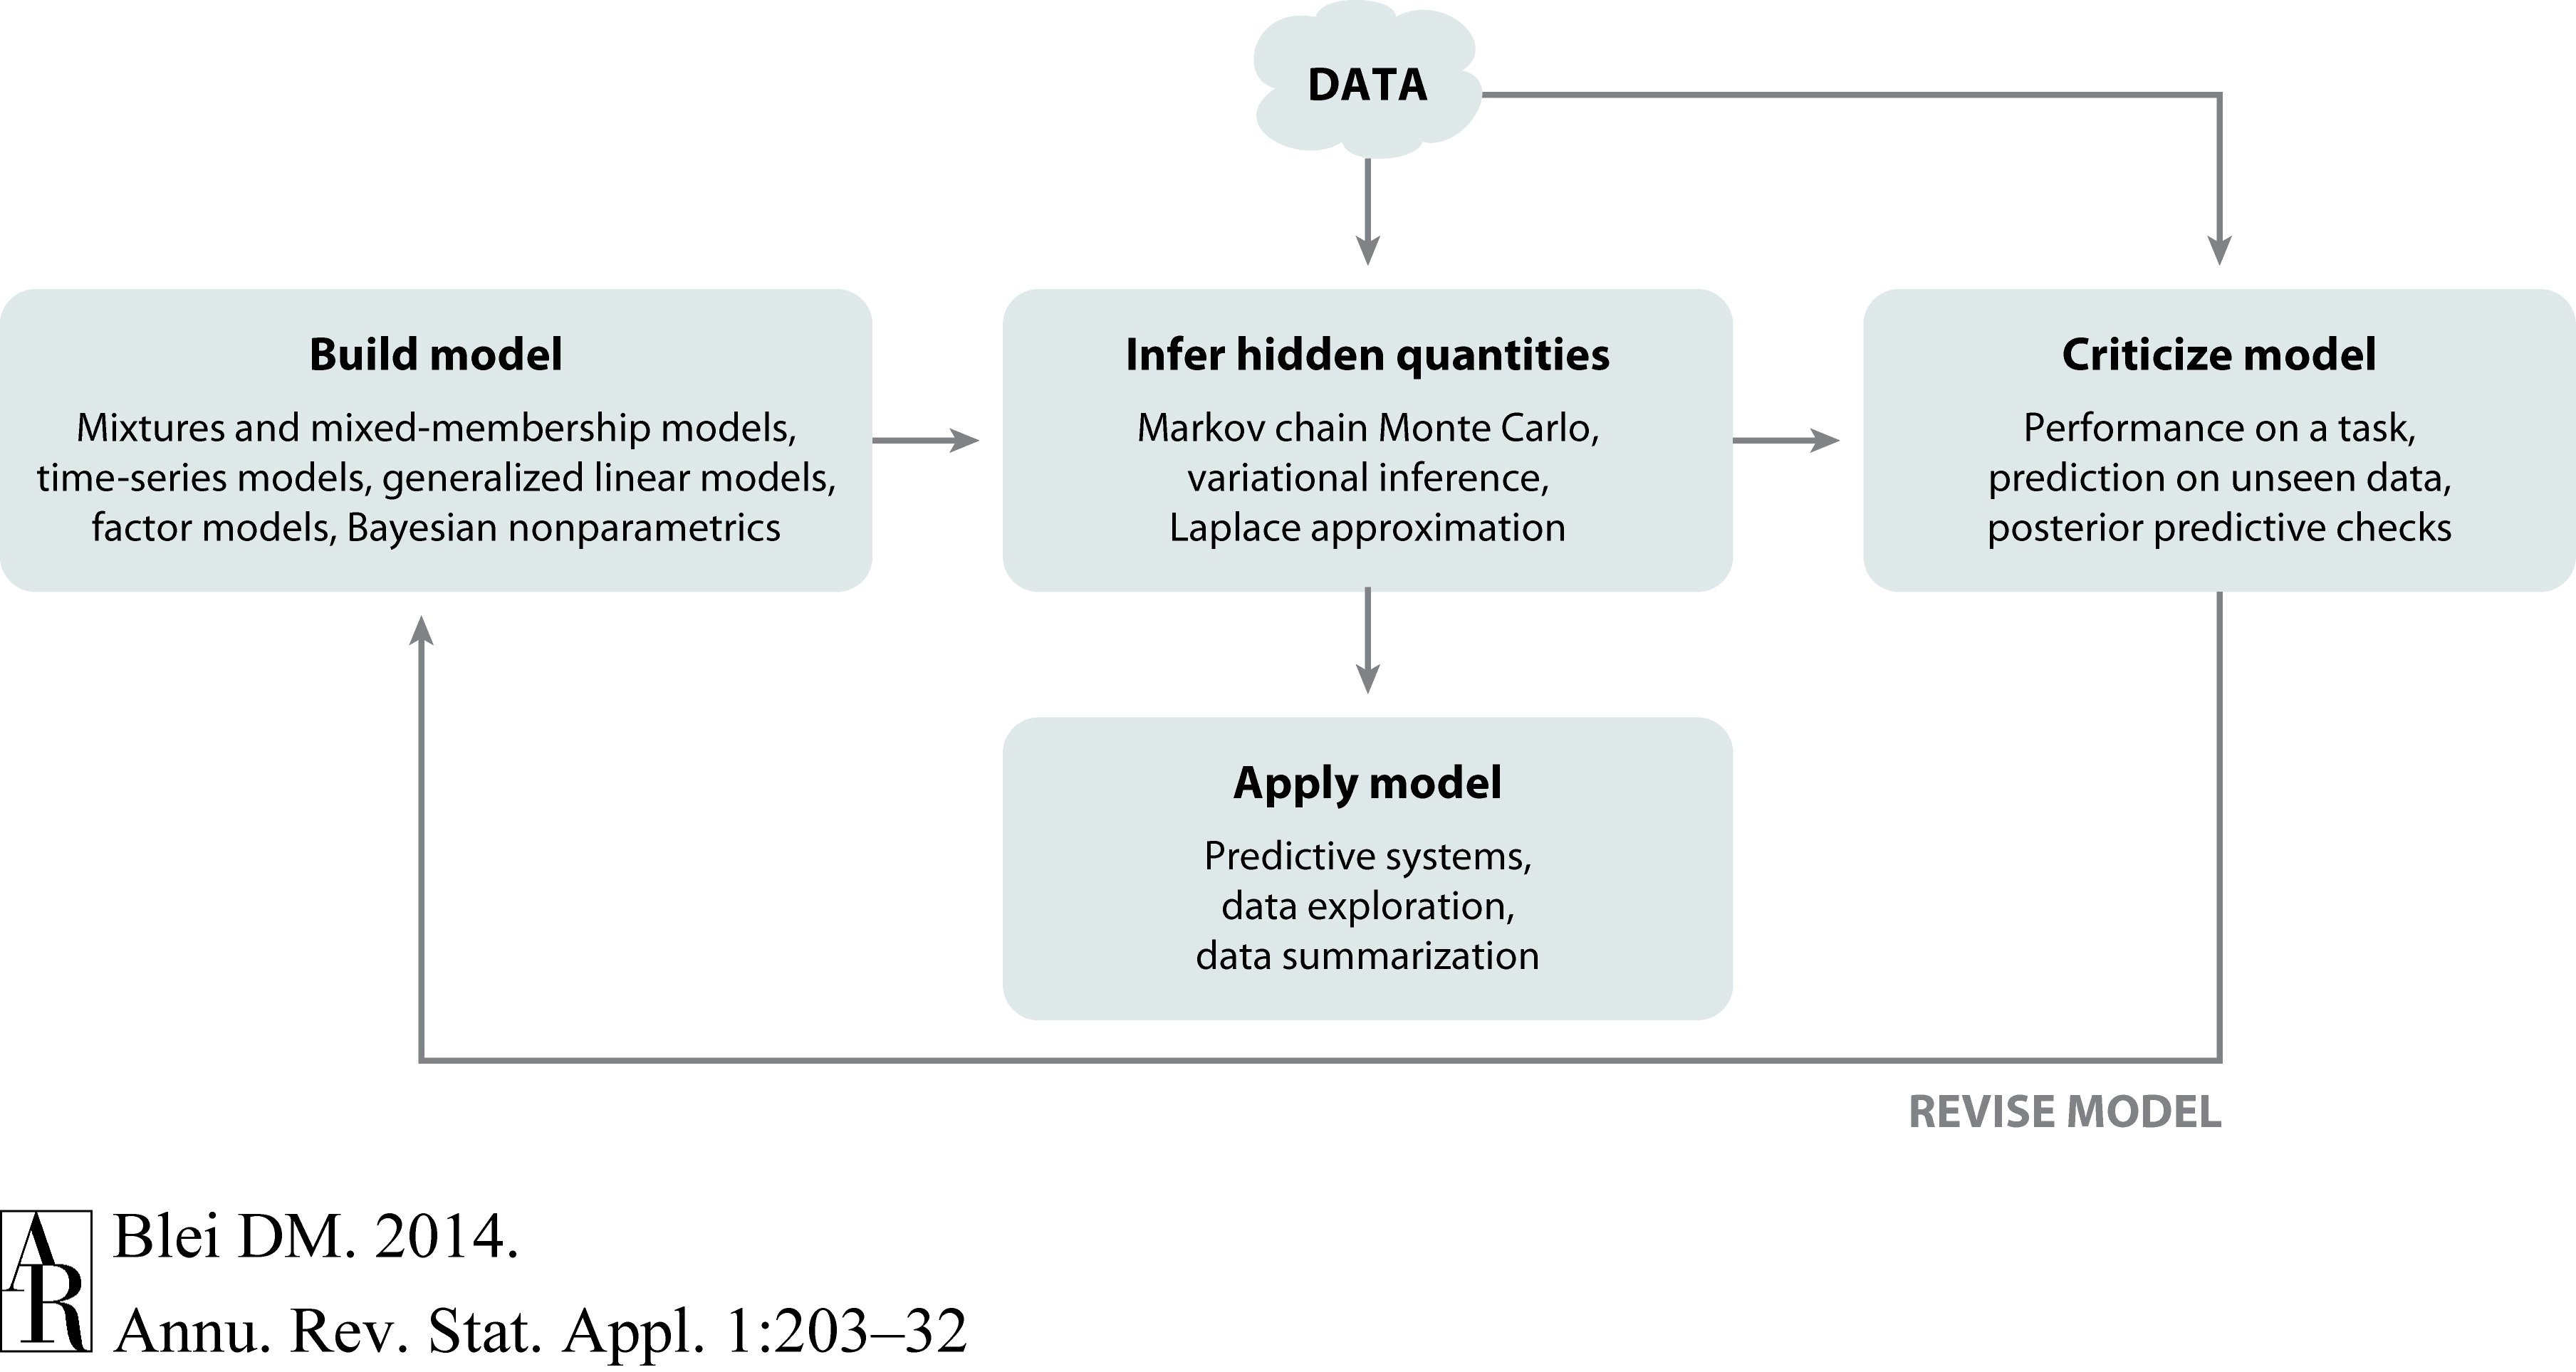
\includegraphics[width=.85\linewidth]{figures/lap1/boxsloop.jpeg}\\
\end{center} 
\begin{flushright}
{\footnotesize Blei, \textit{Ann. Rev. Stat. App.} 2014.}
\end{flushright}
\end{frame}

\begin{frame}{Lap 5: Mixed Membership Models and Variational Inference}
\begin{itemize}
    \item \hyperref[sec:models]{\textbf{Model:} Mixed Membership Models (specifically, topic models)}
    \item \hyperref[sec:cavi]{\textbf{Algorithm:} Coordinate Ascent Variational Inference (CAVI)}
\end{itemize}

\vspace{3em}

\begin{center}
    {\Large \textcolor{red}{These slides are based on unpublished lecture notes by Dave Blei.}}
\end{center}

\end{frame}


\section{Model: Mixed Membership Models}
\label{sec:models}

\begin{frame}{Mixed Membership Models}
    
    Mixed membership models are designed for \textit{grouped data}.
    
    Each ``data point'' is itself a collection of observations. For example,
    \begin{itemize}
        \item in text analysis, a document is a collection of observed words.
        \item in social science, a survey is a collection of observed answers.
        \item in genetic sequencing, a genome is a collection of observed genes.
    \end{itemize}
    
    Mixed membership models look for patterns like the components of a mixture model, but allowing each data point to involve multiple components.
    
\end{frame}


\begin{frame}{Notation for a mixed membership model}
    
\begin{itemize}
    \item Let $\mbx_n = (x_{n,1}, \ldots, x_{n,L})$ denote $n$-th \textbf{data point}. It contains a \textbf{collection of observations}. To simplify notation, assume all data points are length $L$. 

    \item Each data point reflects a \textbf{combination of $K$ mixture components} with parameters $\{\mbeta_k\}_{k=1}^K$. These are shared by all documents.

    \item Each data point has its own \textbf{mixture proportions}, $\mbpi_n \in \Delta_K$.

    \item Each \textbf{observation is assigned to one of the components} by $z_{n,\ell} \in \{1, \ldots, K\}$.
\end{itemize}

\end{frame}


\begin{frame}{Topic models}

The most common mixed-membership model is the \textbf{topic model}, a generative model for documents.

Topic models are so common, they have their own nomenclature:

\begin{table}[]
    \centering
    \begin{tabular}{c|c|c}
        \textit{data set} & \textit{corpus} & collection of documents  \\
        \textit{data point} & \textit{document} & collection of words \\
        \textit{observation} & \textit{word} & one element of a document \\
        \textit{mixture component} & \textit{topic} & distribution over words \\
        \textit{mixture proportions} & \textit{topic proportions} & distribution over topics \\
        \textit{mixture assignment} & \textit{topic assignment} & which topic produced a word \\
    \end{tabular}
    \caption{Rosetta stone for translating between mixed membership model and topic model notation.}
    \label{tab:my_label}
\end{table}
\end{frame}

\begin{frame}{Topic modeling intuition}
\centering
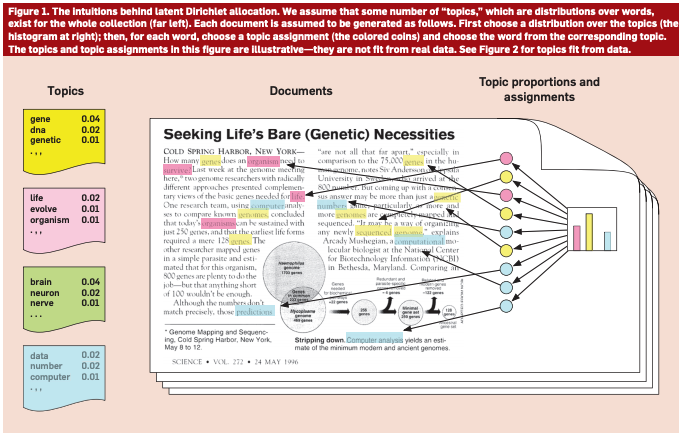
\includegraphics[width=.65\textwidth]{figures/lap5/intuition.png}

From \citet{blei2012probabilistic}.
\end{frame}


\begin{frame}{Topic modeling of New York Times articles}
\centering
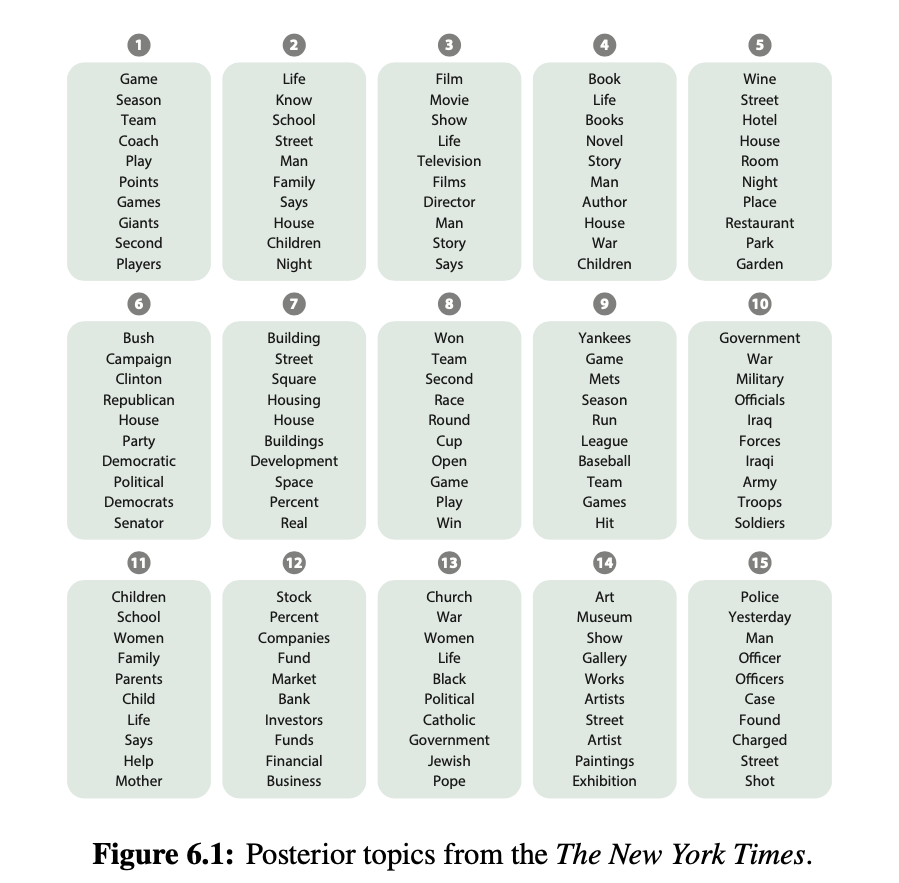
\includegraphics[width=.5\textwidth]{figures/lap5/nyt.png}

\end{frame}


\begin{frame}{Dynamic topic modeling of Science articles}
\centering
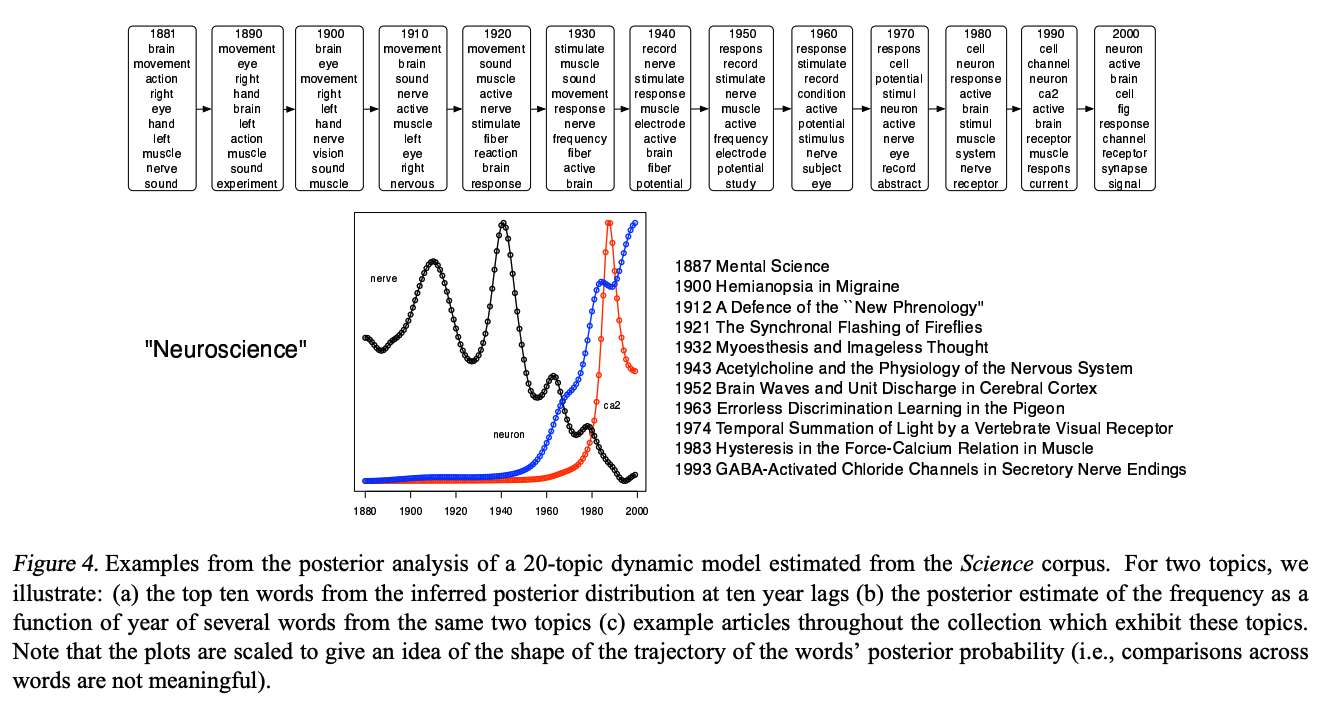
\includegraphics[width=.75\textwidth]{figures/lap5/dtm.png}

From \citet{blei2006dynamic}.
\end{frame}

\begin{frame}{Topic modeling of congressional voting records}
\centering
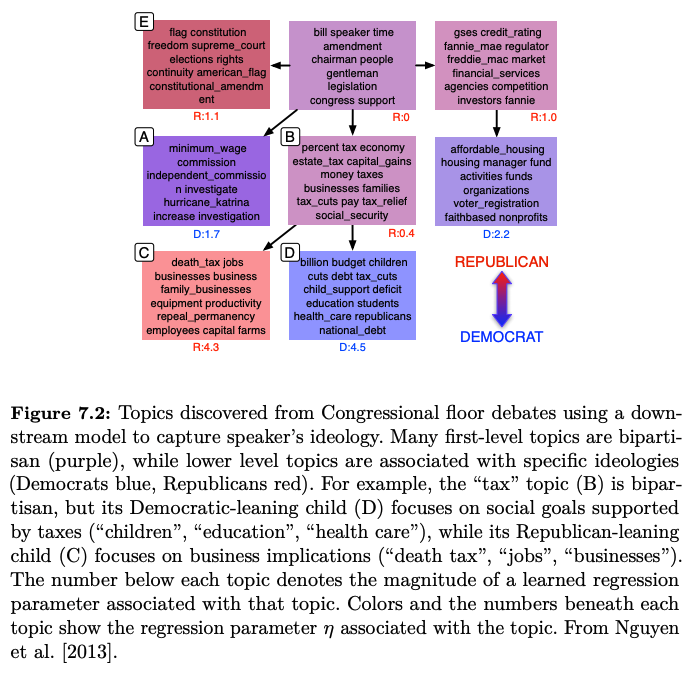
\includegraphics[width=.5\textwidth]{figures/lap5/taxes.png}

From \citet{Boyd-Graber2017-qk}.
\end{frame}


% \begin{frame}{Other applications of topic modeling}
    
%     % Survey data
    
%     % Genetics
    
%     % Behavior data
    
% \end{frame}

\begin{frame}{The generative process for a mixed membership model}
\label{slide:gen_mm}
The generative model process is:
\begin{itemize}
    \item for each mixture component $k = 1, \ldots, K$, sample its parameter $\mbeta_k \sim p(\mbeta_k \mid \mbphi)$
    \item for each data point $n=1,\ldots, N$:
    \begin{itemize}
        \item sample mixture proportions $\mbpi_n \sim \distDirichlet(\mbpi_n \mid \mbalpha)$ 
        \item for each observation $\ell = 1, \ldots, L$:
        \begin{itemize}
            \item sample mixture assignment $z_{n,\ell} \sim \mbpi_n$ 
            \item sample observation $x_{n, \ell} \sim p(x \mid \mbeta_{z_{n,\ell}})$
        \end{itemize}
    \end{itemize}
\end{itemize}
The mixed membership model allows sharing at the dataset level (all data points share the same components) while allowing variability at the data point level (each data point has its own mixture proportions).

\end{frame}

\begin{frame}{The generative process for a topic model}
Slide~\ref{slide:gen_mm} in the language of topic modeling: 
\begin{itemize}
    \item for each \textbf{topic} $k = 1, \ldots, K$, sample its parameter $\mbeta_k \sim p(\mbeta_k \mid \mbphi)$
    \item for each \textbf{document} $n=1,\ldots, N$:
    \begin{itemize}
        \item sample \textbf{topic proportions} $\mbpi_n \sim \distDirichlet(\mbpi_n \mid \mbalpha)$ 
        \item for each \textbf{word} $\ell = 1, \ldots, L$:
        \begin{itemize}
            \item sample \textbf{topic assignment} $z_{n,\ell} \sim \mbpi_n$ 
            \item sample \textbf{word} $x_{n, \ell} \sim p(x \mid \mbeta_{z_{n,\ell}})$
        \end{itemize}
    \end{itemize}
\end{itemize}
The topic model captures sharing at the corpus level (all documents share the same topics) while allowing variability at the data point level (each document weights topics differently).

\end{frame}


\begin{frame}{The joint distribution}
    
The joint probability for a general mixed membership model is,
\begin{align}
p(\{\mbeta_k\}_{k=1}^K, \{\mbpi_n, \mbz_n, \mbx_n\}_{n=1}^N \mid \mbphi, \mbalpha) 
&=
\prod_{k=1}^K p(\mbeta_k \mid \mbphi) 
\prod_{n=1}^N \left[ p(\mbpi_n \mid \mbalpha) 
\prod_{\ell=1}^L p(z_{n,\ell} \mid \mbpi_n) \, p(x_{n,\ell} \mid \mbeta_{z_{n,\ell}}) \right]
\end{align}
As in mixture models, we can write this equivalently as 
\begin{align}
p(\{\mbeta_k\}_{k=1}^K, \{\mbpi_n, \mbz_n, \mbx_n\}_{n=1}^N \mid \mbphi, \mbalpha) 
= 
\prod_{k=1}^K p(\mbeta_k \mid \mbphi) 
\prod_{n=1}^N \left[ p(\mbpi_n \mid \mbalpha) 
\prod_{\ell=1}^L \prod_{k=1}^K \left[\pi_{n,k} \, p(x_{n,\ell} \mid \mbeta_{k})\right]^{\bbI[z_{n,\ell} = k]} \right]
\end{align}
\end{frame}


\begin{frame}[t]{Latent Dirichlet allocation}
    
Latent Dirichlet Allocation (LDA) \citep{blei2003latent} is the most widely used topic model. 

It assumes conjugate Dirichlet-Categorical model for the topics $\mbeta_k$ and words $x_{n,\ell}$,
\begin{align}
    p(\mbeta_k \mid \mbphi) &= \distDirichlet(\mbeta_k \mid \mbphi), \\
    % p(\mbpi_n \mid \mbalpha) &= \distDirichlet(\mbpi_n \mid \mbalpha) \\
    p(x_{n, \ell} \mid \mbeta_{z_{n,\ell}}) &= \mbeta_{z_{n, \ell}, x_{n, \ell}}
\end{align}

Plugging in these assumptions, the joint probability is,
\begin{align}
p(\{\mbeta_k\}_{k=1}^K, & \{\mbpi_n, \mbz_n, \mbx_n\}_{n=1}^N \mid \mbphi, \mbalpha) \\
& = 
\label{eq:lda_joint}
\prod_{k=1}^K \distDirichlet(\mbeta_k \mid \mbphi) 
\prod_{n=1}^N \left[ \distDirichlet(\mbpi_n \mid \mbalpha) 
\prod_{\ell=1}^L \pi_{n,z_{n,\ell}} \, \eta_{z_{n,\ell},x_{n,\ell}} \right] \\
% & = 
% \prod_{k=1}^K \distDirichlet(\mbeta_k \mid \mbphi) 
% \prod_{n=1}^N \left[ \distDirichlet(\mbpi_n \mid \mbalpha) 
% \prod_{\ell=1}^L \prod_{k=1}^K \left[\pi_{n,k} \, \eta_{k,x_{n,\ell}} \right]^{\bbI[z_{n,\ell} = k]} \right] \\
& = 
\prod_{k=1}^K \distDirichlet(\mbeta_k \mid \mbphi) 
\prod_{n=1}^N \Bigg( \distDirichlet(\mbpi_n \mid \mbalpha) 
\prod_{\ell=1}^L \left[ \prod_{k=1}^K \pi_{n,k}^{\bbI[z_{n,\ell} = k]} \right] \left[ \prod_{k=1}^K \prod_{v=1}^V \eta_{k,v}^{\bbI[z_{n,\ell}=k] \bbI[x_{n,\ell} = v]} \right] \Bigg)
\end{align}
\end{frame}

\begin{frame}{Gibbs sampling for LDA}
\label{slide:gibbs}
As usual, sample each variable from its conditional distribution, holding the rest fixed.

\begin{itemize}
    \item<1-> \textbf{Topic assignments:} The assignments are conditionally independent given the topic parameters and proportions,
    \begin{align}
        p(z_{n,\ell} \mid \mbx_n, \{\mbeta_k\}_{k=1}^K, \mbpi_n) &\propto \pi_{n, z_{n, \ell}} p(x_{n, \ell} \mid \mbeta_{z_{n, \ell}})
    \end{align}
    
    \item<2-> \textbf{Topic proportions: } Let $N_{n,k} = \sum_{\ell=1}^L \bbI[z_{n,\ell} = k]$ denote the number of words in document $n$ assigned to topic $k$. Then,
    \begin{align}
        p(\mbpi_n \mid \mbalpha, \mbz_n) &\propto \distDirichlet(\mbpi_n \mid \mbalpha) \prod_{k=1}^K \pi_{n,k}^{N_{n,k}} = \distDirichlet([\alpha_1 + N_{n,1}, \ldots, \alpha_K + N_{n,K}]).
    \end{align}
    
    \item<3-> \textbf{Topic parameters: } Let $N_{k,v} = \sum_{n=1}^N \sum_{\ell=1}^L \bbI[z_{n,\ell}=k] \bbI[x_{n,\ell}=v]$ denote the number of times word~$v$ was assigned to topic $k$ across all documents. Then,
\begin{align}
    p(\mbeta_k \mid \{\mbz_n, \mbx_n\}, \mbphi) &\propto
    \distDirichlet(\mbeta_k \mid \mbphi) \prod_{v=1}^V \eta_{k,v}^{N_{k,v}} = \distDirichlet([\phi_1 + N_{k,v}, \ldots, \phi_V + N_{k,V}]).
\end{align}

\end{itemize}
\end{frame}

\begin{frame}{Why does LDA produce sharp topics?}
Consider the log posterior as a function of $\mbeta_k$ and $\mbpi_n$. From eq.~\ref{eq:lda_joint}, it is,
\begin{align}
    \sum_{k=1}^K \log p(\mbeta_k \mid \mbphi) + \sum_{n=1}^N \log p(\mbpi_n \mid \mbalpha) + \sum_{n=1}^N \sum_{\ell=1}^L \left( \log \pi_{n, z_{n, \ell}} + \log \eta_{z_{n, \ell}, x_{n, \ell}} \right)
\end{align}
The double sum over $n$ and $\ell$ dominates this expression.

It encourages topic proportions and topic probabilities to both be large, but recall that both $\mbpi_n$ and $\mbeta_k$ are constrained to the simplex.

For $\log \pi_{n,z_{n,\ell}}$ to be large, the posterior should assign all words to as few topics as possible. 

For $\log \eta_{z_{n,\ell}, x_{n, \ell}}$ to be large, the topics should put high probability on as few words as possible.

These goals are at odds. The LDA posterior balances these goals to find topics with sharply co-occuring words.

\end{frame}

% \begin{frame}{From words to word counts}

% So far we've treated documents as a sequence of discrete words, but note that all we really needed were the word counts $N_{n,v} = \sum_{\ell=1}^L \bbI[x_{n,\ell} = v]$
    
% \end{frame}

\section{Algorithm: CAVI}
\label{sec:cavi}

\begin{frame}{Lap 5: Mixed Membership Models and Variational Inference}
\begin{itemize}
    \item \hyperref[sec:models]{Model: Mixed Membership Models}
    \item \hyperref[sec:cavi]{\textbf{Algorithm: Coordinate Ascent Variational Inference (CAVI)}}
\end{itemize}
\end{frame}

\begin{frame}{Taking stock}
    
We've covered a number of posterior inference algorithms thus far:
\begin{itemize}
    \item \textbf{Exact inference:} for simple models (e.g. conjugate exponential family models) where the posterior is available in closed form.
    
    \item \textbf{Laplace approximation:} approximate the posterior with a Gaussian centered on the posterior mode that matches the local curvature. This works well for sharp, unimodal posteriors over continuous latent variables.
    
    \item \textbf{Metropolis-Hastings: } a very general MCMC algorithm to sample the posterior, and the building block for many other MCMC techniques.
    
    \item \textbf{Hamiltonian Monte Carlo: } an MCMC algorithm to draw samples from the posterior by leveraging gradients of the log joint probability. This works well for more general posteriors over continuous variables.
    
    \item \textbf{Gibbs sampling:} an MCMC algorithm that iteratively samples conditional distributions for one variable at a time. This works well for conditionally conjugate models with weak correlations.
\end{itemize}
\end{frame}

\begin{frame}{Variational inference}

We liked the Laplace approximation because they were deterministic and often very efficient to compute, but they were biased for non-Gaussian posteriors.

MCMC methods are asymptotically unbiased (though for finite samples there is a transient bias that shrinks as $O(S^{-1})$. The real issue is variance: it only shrinks as $O(S^{-1/2})$.

\textbf{Motivation: } With finite computation, can we get better posterior estimates by trading asymptotic bias for smaller variance? 

\textbf{Idea: } approximate the posterior by with a simple, parametric form (though not strictly a Gaussian on the mode!). Optimize to find the approximation that is as ``close'' as possible to the posterior.
    
\end{frame}

\begin{frame}{Notation}
Let,
\begin{itemize}
    \item $\mbtheta \in \reals^P$ denote the collection of latent variables and parameters we wish to infer. \\
    In LDA, $\mbtheta = \{\mbeta_k\}_{k=1}^K, \{\mbpi_n, \mbz_n\}_{n=1}^N$.
    
    \item $p(\mbtheta \mid \mbx)$ denote the posterior distribution we want to approximate.
    
    \item $q(\mbtheta; \mblambda)$ denote a parametric \textit{variational approximation} to the posterior where...
    
    \item $\mblambda$ denotes the \textit{variational parameters} that we will optimize.
    
    \item $D(q \, \| \, p)$ denote a \textit{divergence measure} that takes in two distributions $q$ and $p$ and returns a measure of how similar they are.
\end{itemize}
\end{frame}

\begin{frame}{A view of variational inference}
\centering
    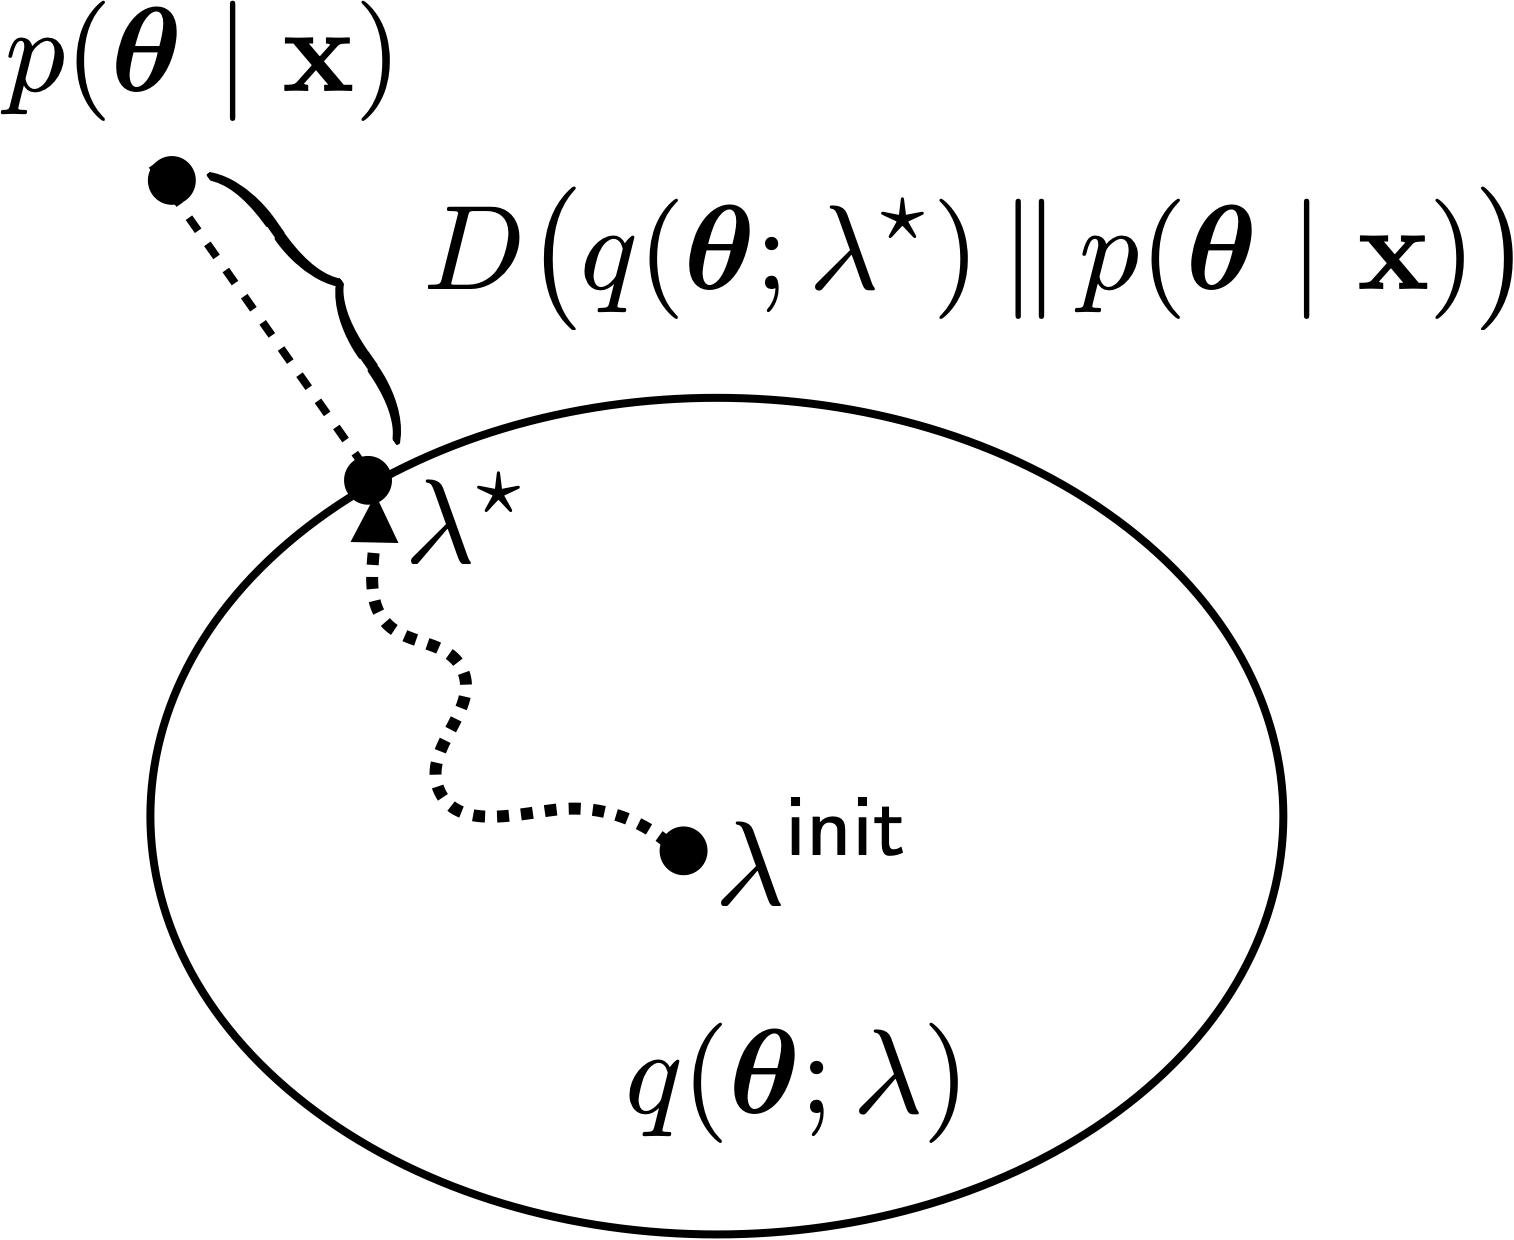
\includegraphics[width=.5\textwidth]{figures/lap5/vi.png}
\end{frame}

\begin{frame}{Key questions}
\begin{itemize}
    \item \textit{What parametric family should we use? }
    \begin{itemize}
        \item This lecture: the \textbf{mean-field family}.
    \end{itemize}
    
    \item \textit{How should we measure closeness? }
    \begin{itemize}
        \item This lecture: the \textbf{Kullback-Leibler (KL)} divergence.
    \end{itemize}
    
    \item \textit{How do we find the closest distribution in that family?}
    \begin{itemize}
        \item This lecture: \textbf{coordinate ascent.}
    \end{itemize}
\end{itemize}

These choices are what \citet{Blei2017-yc} call \textbf{coordinate ascent variational inference}~CAVI).
\end{frame}

\begin{frame}{The mean-field family}
The \textit{mean-field family} gets its name from statistical mechanics. It treats each latent variable and parameter as independent with its own variational parameter,
\begin{align}
    q(\mbtheta; \mblambda) &= \prod_{j=1}^P q(\theta_j; \lambda_j).
\end{align}

For example, in LDA the mean field approximation treats each topic, topic proportion, and topic assignment as independent,
\begin{align}
    q(\{\mbeta_k\}_{k=1}^K, \{\mbpi_n, \mbz_n\}_{n=1}^N; \mblambda) &= \prod_{k=1}^K q(\mbeta_k; \mblambda_k^{(\mbeta)}) 
    \prod_{n=1}^N q(\mbpi_n; \mblambda_n^{(\mbpi)}) 
    \prod_{n=1}^N \prod_{\ell=1}^L q(z_{n, \ell}; \mblambda_{n, \ell}^{(z)})
\end{align}

\textbf{Question: } Is this a good approximation to the posterior? 

\end{frame}

\begin{frame}{The Kullback-Leibler (KL) divergence}
The KL divergence is a measure of closeness between two distributions. It is defined as,
\begin{align}
    \KL{q(\mbtheta; \mblambda)}{p(\mbtheta \mid \mbx} &= \E_{q(\mbtheta; \mblambda)} \left[ \log \frac{q(\mbtheta; \mblambda)}{p(\mbtheta \mid \mbx)} \right] \\
    &= \E_{q(\mbtheta; \mblambda)} \left[ \log q(\mbtheta; \mblambda) \right] 
    - \E_{q(\mbtheta; \mblambda)} \left[ \log p(\mbtheta \mid \mbx) \right] 
    % \\
    % &= \underbrace{\bbH[q(\mbtheta; \mblambda), p(\mbtheta \mid \mbx)]}_{\text{cross entropy}} - \underbrace{\bbH[q(\mbtheta; \mblambda)]}_{\text{entropy}}
\end{align}

It has some nice properties:
\begin{itemize}
    \item It is non-negative.
    
    \item It is zero iff $q(\mbtheta; \mblambda) \equiv p(\mbtheta \mid \mbx)$.
    
    \item It is defined in terms of expectations wrt $q$.
\end{itemize}

But it's also a bit weird... 
\begin{itemize}
    \item It's asymmetric ($\KL{q}{p} \neq \KL{p}{q}$).
\end{itemize}
\end{frame}

\begin{frame}{The evidence lower bound (ELBO)}
    More concerning, the KL divergence involves the posterior $p(\mbtheta \mid \mbx)$, which we cannot compute!
    
    But notice that...
    \begin{align}
        \KL{q(\mbtheta; \mblambda)}{p(\mbtheta \mid \mbx}
        &= \E_{q(\mbtheta; \mblambda)} \left[ \log q(\mbtheta; \mblambda) \right] 
        - \E_{q(\mbtheta; \mblambda)} \left[ \log p(\mbtheta \mid \mbx) \right] \\
        &= \E_{q(\mbtheta; \mblambda)} \left[ \log q(\mbtheta; \mblambda) \right] 
        - \E_{q(\mbtheta; \mblambda)} \left[ \log p(\mbtheta, \mbx) \right] 
        + \E_{q(\mbtheta; \mblambda)}\left[ \log p(\mbx)\right] \\
        &= \underbrace{\E_{q(\mbtheta; \mblambda)} \left[ \log q(\mbtheta; \mblambda) \right] 
        - \E_{q(\mbtheta; \mblambda)} \left[ \log p(\mbtheta, \mbx) \right]}_{\text{negative ELBO}, -\cL(\mblambda)}
        + \underbrace{\log p(\mbx)}_{\text{evidence}}
    \end{align}
The first term involves the log joint, which we can compute, and the last term is independent of the variational parameters! 

Rearranging, we see that $\cL(\mblambda)$ is a lower bound on the marginal likelihood, aka the evidence,
\begin{align}
    \cL(\mblambda) &= \log p(\mbx) - \KL{q(\mbtheta; \mblambda)}{p(\mbtheta \mid \mbx} 
    \leq \log p(\mbx).
\end{align}
That's why we call it the \textbf{evidence lower bound (ELBO)}.
\end{frame}

\begin{frame}{Viewer discretion advised...}
    
    \centering
    % \includemedia[
    %     width=0.75\linewidth,height=0.3375\linewidth, % 16:9
    %     activate=pageopen,
    %     flashvars={
    %     modestbranding=1 % no YT logo in control bar
    %     &autohide=1 % controlbar autohide
    %     &showinfo=0 % no title and other info before start
    %     &rel=0 % no related videos after end
    %     }
    %     ]{}{https://www.youtube.com/watch?v=jugUBL4rEIM}
    \url{https://www.youtube.com/watch?v=jugUBL4rEIM}
    
\end{frame}

\begin{frame}{Optimizing the ELBO with coordinate ascent}
We want to find the variational parameters $\mblambda$ that minimize the KL divergence or, equivalently, maximize the ELBO.

For the mean-field family, we can typically do this via \textbf{coordinate ascent}. 

Consider optimizing the parameters for one factor~$q(\theta_j; \lambda_j)$. As a function of $\lambda_j$, the ELBO is,
\begin{align}
    \cL(\mblambda) 
    &= 
    \E_{q(\theta_j; \lambda_j)}\left[ \E_{q(\mbtheta_{\neg j}; \mblambda_{\neg j})} \left[ \log p(\mbtheta, \mbx) \right] \right] -
    \E_{q(\theta_j; \lambda_j)}[\log q(\theta_j; \lambda_j)] + c \\
    &= 
    \E_{q(\theta_j; \lambda_j)}\left[ \E_{q(\mbtheta_{\neg j}; \mblambda_{\neg j})} \left[ \log p(\theta_j \mid \mbtheta_{\neg_j}, \mbx) \right] \right] -
    \E_{q(\theta_j; \lambda_j)}[\log q(\theta_j; \lambda_j)] + c' \\
    &= -\KL{q(\theta_j; \lambda_j)}{\tilde{p}(\theta_j)} + c''
\end{align}
where 
\begin{align}
    \label{eq:cavi_form}
    \tilde{p}(\theta_j) &\propto
    \exp \left\{ \E_{q(\mbtheta_{\neg j}; \mblambda_{\neg j})} \left[ \log p(\theta_j \mid \mbtheta_{\neg j}, \mbx) \right] \right\}
\end{align}
The ELBO is maximized wrt $\lambda_j$ when this KL is minimized; i.e. when $q(\theta_j ; \lambda_j) = \tilde{p}(\theta_j)$, the exponentiated expected log conditional probability, holding all other factors fixed.
\end{frame}

% \begin{frame}{Next time}
%     \begin{itemize}
%         \item Coordinate ascent variational inference for LDA
%         \item Word count formulation
%         \item Evaluating topic models and choosing $K$
%         \item Stochastic variational inference
%     \end{itemize}
% \end{frame}

\subsection{CAVI for LDA}
\label{sec:cavi_lda}

\begin{frame}{Lap 5: Mixed Membership Models and Variational Inference}
\begin{itemize}
    \item \hyperref[sec:models]{Model: Mixed Membership Models}
    \item \hyperref[sec:cavi]{Algorithm: Coordinate Ascent Variational Inference (CAVI)}
    \begin{itemize}
        \item \textbf{CAVI for LDA}
    \end{itemize}
\end{itemize}
\end{frame}

\begin{frame}{Coordinate Ascent Variational Inference for LDA}

Let's derive the CAVI updates for LDA.

Assume a mean field family, and assume each factor is of the same exponential family form as the corresponding prior:
\begin{align}
    q(z_{n,\ell}; \mblambda^{(z)}_{n, \ell}) &= \distCategorical(z_{n, \ell}; \mblambda^{(z)}_{n, \ell}) \\
    q(\mbpi_n; \mblambda^{(\mbpi)}_{n}) &= \distDirichlet(\mbpi_n; \mblambda^{(\mbpi)}_{n}) \\
    q(\mbeta_k; \mblambda^{(\mbeta)}_{k}) &= \distDirichlet(\mbeta_k; \mblambda^{(\mbeta)}_{k}).
\end{align}
so $\mblambda^{(z)}_{n, \ell} \in \Delta_K$, $\mblambda^{(\mbpi)}_{n} \in \reals_+^K$, and $\mblambda^{(\mbeta)}_{k} \in \reals_+^V$ are the variational parameters.

(It turns out, for conjugate exponential family models, the optimal variational factors are of the same form as the prior anyway!)
\end{frame}

\begin{frame}{CAVI updates for the topic assignments}
Recall that the optimal CAVI updates are of the form in Eq.~\ref{eq:cavi_form}. 

We already derived the conditional distributions for Gibbs sampling (Slide~\ref{slide:gibbs}).

For the topic assignments, the CAVI update is,
\begin{align}
    \log q(z_{n, \ell} = k; \mblambda^{(z)}_{n, \ell}) &=
    \E_{q(\mbpi_n) q(\mbeta_k)} \left[ \log \pi_{n, k} + \log p(x_{n, \ell} \mid \eta_{k}) \right] + c \\
    &= \E_{q(\mbpi_n)} \left[ \log \pi_{n, k} \right] + \E_{q(\mbeta_k)} \left[ \log \eta_{k, x_{n, \ell}} \right] + c \\
    &= \log \distCategorical(z_{n, \ell} = k; \mblambda^{(z)}_{n, \ell}) \\
    \Rightarrow \log \lambda_{n,\ell,k}^{(z)} &= \E_{q(\mbpi_n)} \left[ \log \pi_{n, k} \right] + \E_{q(\mbeta_k)} \left[ \log \eta_{k, x_{n, \ell}} \right] + c
\end{align}
Since $\mblambda_{n,\ell}^{(z)}$ must sum to one,
\begin{align}
\label{eq:q_z_update}
\lambda_{n,\ell,k}^{(z)} &= \frac{\exp\left\{\E_{q(\mbpi_n)} \left[ \log \pi_{n, k} \right] + \E_{q(\mbeta_k)} \left[ \log \eta_{k, x_{n, \ell}} \right]\right\}}{\sum_{j=1}^K \exp\left\{\E_{q(\mbpi_n)} \left[ \log \pi_{n, j} \right] + \E_{q(\mbeta_j)} \left[ \log \eta_{j, x_{n, \ell}} \right]\right\} }
\end{align}
\end{frame}

\begin{frame}{Expectations under Dirichlet distributions}
The variational factors for $\mbpi_n$ and $\mbeta_k$ are Dirichlet distributions. 

The necessary expectations have closed form expressions:
\begin{align}
    \E_{\distDirichlet(\mbpi; \mbalpha)}[\log \pi_k] = \psi(\alpha_k) - \psi \Big(\sum_{j=1}^K \alpha_j \Big)
\end{align}
where $\psi(\cdot)$ is the \emph{digamma function}, the logarithmic derivative of the gamma function.
\end{frame}

\begin{frame}{CAVI updates for the topic proportions}
Referring back to Slide~\ref{slide:gibbs}, we see the CAVI update is,
\begin{align}
    \log q(\mbpi_{n}; \mblambda^{(\mbpi)}_{n}) &=
    \E_{q(\mbz_n)} \left[ \log \distDirichlet(\mbpi_n; \mbalpha) + \sum_{k=1}^K N_{n,k} \log \pi_{n,k} \right] + c \\
    &= \sum_{k=1}^K (\alpha_k - 1 + \E_{q(\mbz_n)}[N_{n,k}]) \log \pi_{n,k} \\
    &= \log \distDirichlet\Big(\mbpi_n; \mblambda_n^{(\mbpi)} \Big) \\
    \Rightarrow \mblambda^{(\mbpi)}_n &= \Big[\alpha_1 + \E_{q(\mbz_n)}[N_{n,1}], \ldots, \alpha_1 + \E_{q(\mbz_n)}[N_{n,K}] \Big],
\end{align}
where
\begin{align}
    \E_{q(\mbz_n)}[N_{n,k}] 
    &= \sum_{\ell=1}^L \E_{q(z_{n,\ell})}[\bbI[z_{n,\ell}=k]]
    = \sum_{\ell=1}^L \lambda_{n,\ell,k}^{(z)}.
\end{align}
\end{frame}

\begin{frame}{CAVI updates for the topic parameters}
The topic parameter updates are similar
\begin{align}
    \log q(\mbeta_k; \mblambda^{(\mbeta)}_k) &=
    \E_{q(\mbz)} \left[ \log \distDirichlet(\mbeta_k; \mbphi) + \sum_{v=1}^V N_{k,v} \log \eta_{k,v} \right] + c \\
    &= \sum_{v=1}^V (\phi_v - 1 + \E_{q(\mbz)}[N_{k,v}]) \log \eta_{k,v} \\
    &= \log \distDirichlet\Big(\mbeta_k; \mblambda^{(\mbeta)}_k \Big) \\
    \Rightarrow \mblambda^{(\mbeta)}_k &= \Big[\phi_1 + \E_{q(\mbz)}[N_{k,1}], \ldots, \phi_1 + \E_{q(\mbz)}[N_{k,V}] \Big],
\end{align}
where
\begin{align}
    \E_{q(\mbz)}[N_{k,v}] 
    &= \sum_{n=1}^N \sum_{\ell=1}^L \E_{q(z_{n,\ell})}[\bbI[z_{n,\ell}=k]]
    = \sum_{n=1}^N \sum_{\ell=1}^L \lambda_{n,\ell,k}^{(z)}.
\end{align}
\end{frame}

\begin{frame}{Calculating the ELBO}
Dropping hyperparameters and variational parameters, the ELBO is,
\begin{align}
    \cL(\mblambda) &= \E_{q}[\log p(\{\mbx_n, \mbz_n, \mbpi_n\}_{n=1}^N, \{\mbeta_k\}_{k=1}^K)] - \E_q[\log q(\{\mbz_n, \mbpi_n\}_{n=1}^N, \{\mbeta_k\}_{k=1}^K)] 
\end{align}
Thanks to the factorization of the joint distribution and the variational posterior, this simplifies,
\begin{multline}
    \cL(\mblambda) = \sum_{n=1}^N \E_{q}[\log p(\mbpi_n)] + \sum_{k=1}^K \E_q[\log p(\mbeta_k)] \\
    + \sum_{n=1}^N \sum_{\ell=1}^L \E_q[\log p(z_{n,\ell} \mid \mbpi_n)] + \E_q[\log p(x_{n, \ell} \mid z_{n,\ell}, \mbeta)] \\
    -\sum_{k=1}^K \E_q[\log q(\mbeta_k)] - \sum_{n=1}^N \E_q[\log q(\mbpi_n)]
    -\sum_{n=1}^N \sum_{\ell=1}^L \E_q[\log q(z_{n, \ell})]
\end{multline}
The first two terms are Dirichlet cross entropies and the last three terms are entropies. Tensorflow probability has already implemented these functions for you, so this is easier to calculate than you might think!
\end{frame}

\begin{frame}{Calculating the ELBO II}
The middle terms are,
\begin{align}
    \E_q[\log p(z_{n,\ell} \mid \mbpi_n)] 
    &= \sum_{k=1}^K \E_{q(z_{n,\ell})}[\bbI[z_{n,\ell}=k]] \cdot \E_{q(\mbpi_n)} [\log \pi_{n,k}] \\
    &= \sum_{k=1}^K \lambda_{n,\ell,k}^{(z)} \cdot \E_{q(\mbpi_n)} [\log \pi_{n,k}]
\end{align}
and
\begin{align}
    \E_q[\log p(x_{n, \ell} \mid z_{n,\ell}, \mbeta)] 
    &= \sum_{k=1}^K \E_{q(z_{n,\ell})}[\bbI[z_{n,\ell}=k]] \cdot \E_{q(\mbeta_k)} [\log \eta_{k,x_{n,\ell}}] \\
    &= \sum_{k=1}^K \lambda_{n,\ell,k}^{(z)} \cdot \E_{q(\mbeta_k)} [\log \eta_{k,x_{n,\ell}}] 
\end{align}
Again, these involve only simple expectations of Dirichlet distributions.
\end{frame}

\begin{frame}{Bag of word counts representation and exchangeability}

LDA models the words as \textbf{exchangeable} random variables. That is, the joint distribution is invariant to permutations:
\begin{align}
    p(\mbx_n) = p(x_{n,1}, \ldots, x_{n,L}) \equiv
    p(x_{n,\sigma(1)}, \ldots, p(x_{n,\sigma(L)})) 
\end{align}
where $\sigma(\cdot)$ is any permutation of the indices $\{1,\ldots,L\}$.

In text modeling, this is called the \textbf{bag of words} assumption.

\textbf{De Finetti's theorem} says that any joint distribution over exchangeable random variables can be represented as a marginal of \textit{some} latent variable model of the form,
\begin{align}
    p(\mbx_n) &= \int p(\theta) \prod_{\ell=1}^L p(x_{n,\ell} \mid \theta) \dif \theta.
\end{align}
This is one justification for the \textbf{conditional independence assumptions} we often make in Bayesian models.


\end{frame}

\begin{frame}{CAVI updates in the bag-of-words representation}

We can use the exchangeability assumption to work with word counts rather than word indicators. 

Note that $\lambda_{n,\ell,k}^{(z)} = \lambda_{n,\ell',k}^{(z)}$ if $x_{n,\ell} = x_{n,\ell'}$. Instead of having parameters for each word instance~$\ell$, zhave one for each term~$v$ in the vocabulary,
\begin{align}
\lambda_{n,v,k}^{(z)} &= \frac{\exp\left\{\E_{q(\mbpi_n)} \left[ \log \pi_{n, k} \right] + \E_{q(\mbeta_k)} \left[ \log \eta_{k, v} \right]\right\}}{\sum_{j=1}^K \exp\left\{\E_{q(\mbpi_n)} \left[ \log \pi_{n, j} \right] + \E_{q(\mbeta_j)} \left[ \log \eta_{j, v} \right]\right\} }
\end{align}

Then let $y_{n,v} = \sum_{\ell=1}^L \bbI[x_{n,\ell}=v]$ denote the number of instances of word $v$ in document $n$.

From these variational parameters, it's easy to compute the expected summary counts,
\begin{align}
    \E_{q}[N_{n,k}] &= \sum_{v=1}^V y_{n,v} \lambda^{(z)}_{n,v,k} 
    &
    \E_{q}[N_{k,v}] &= \sum_{n=1}^N y_{n,v} \lambda^{(z)}_{n,v,k} 
\end{align}
\end{frame}

\begin{frame}{Scaling up to very large datasets}

There are a few tricks to make LDA much more scalable. 

First, to save memory, you only need to track, $\mblambda_{n,v}^{(z)} = [\lambda_{n,v,1}^{(z)}, \ldots, \lambda_{n,v,K}^{(z)}]$ if $y_{n,v} > 0$. 

Likewise, you can process documents in rolling fashion, discarding $\mblambda_{n,v}^{(z)}$ once you've updated $\E_q[N_{k,v}]$ and $\mblambda_n^{(\mbpi)}$. 

Finally, you can use \textbf{stochastic variational inference} \citep{hoffman2013stochastic} to work with mini-batches of documents to get Monte Carlo estimates of $\E_q[N_{k,v}]$. 

SVI can be seen as \textbf{stochastic gradient ascent} on the ELBO using \textbf{natural gradients} \citet{amari1998natural}; i.e., gradient descent preconditioned with the Fisher information matrix.

    
\end{frame}

\begin{frame}{Evaluating topic models}
    
The key hyperparameter is $K$, the number of topics. By now, we've seen a few different ways of setting these ``complexity knobs.'' 

\textbf{Question: } what approaches could we take?

Blei recommends another method that differs slightly from what we've seen thus far. He suggests evaluating,
\begin{align}
    p(\mbx_{n'}^{\mathsf{out}} \mid \mbx_{n'}^{\mathsf{in}}, \{\mbx_n\}_{n=1}^N) 
    &= \int p(\mbx_{n'}^{\mathsf{out}} \mid \mbpi_{n'}, \{\mbeta_k\}_{k=1}^K) \, p(\mbpi_{n'} \mid \mbx_{n'}^{\mathsf{in}}, \{\mbeta_k\}_{k=1}^K) \, p(\{\mbeta_k\}_{k=1}^K \mid \{\mbx_n\}_{n=1}^N) \dif \mbpi_{n'}
\end{align}
where 
\begin{itemize}
    \item $\mbx_{n'}^{\mathsf{out}}$ consists of a subset of words in a held-out document $n'$
    \item $\mbx_{n'}^{\mathsf{in}}$ are the remaining words in that document, which are used to estimate the topic proportions, and
    \item $\{\mbx_n\}_{n=1}^N$ are the training documents used to estimate the topics $\{\mbeta_k\}_{k=1}^K$.
\end{itemize}
\citet{wallach2009evaluation} discuss topic model evaluation in detail.
\end{frame}

\begin{frame}[t]{Evaluating topic models II}
\textbf{Question: } why not simply compare the ELBO for different values of $K$? It's related to the marginal likelihood, after all. 
\end{frame}


\begin{frame}{Other mixed membership models}
\begin{itemize}
    \item LDA evolved from a long line of work on topic modeling. \citet{Deerwester1990-kp} proposed \textbf{latent semantic analysis} and \citet{Hofmann1999-de} proposed a probabilistic version called the \textbf{aspect model}.
    
    \item \citet{Pritchard2000-wm} developed MM models in \textbf{population genetics}.
    
    \item \citet{Erosheva2007-vd} used MM models for \textbf{survey data}.
    
    \item \citet{Airoldi2008-rh} developed MM models for \textbf{community detection in networks}. \citet{Gopalan2013-pz} developed a stochastic variational inference algorithm for this model.
    
    \item \citet{Gopalan2013-bc} proposed \textbf{Poisson matrix factorization}, which is closely related to LDA. 
\end{itemize}
\end{frame}

\begin{frame}[t,allowframebreaks]
        \frametitle{References}
        \bibliographystyle{unsrtnat}
        \bibliography{refs.bib}
\end{frame}

\end{document}